\documentclass[12pt,preprint,times]{elsarticle}
%\usepackage{graphicx}
\usepackage{xcolor}
\usepackage{multirow}
\usepackage[utf8]{inputenc}
%\usepackage[ansinew]{inputenc}
\usepackage[psamsfonts]{amssymb}
\usepackage{amsmath}
\usepackage[all]{xy}
\usepackage{graphicx}
\usepackage{float}
\usepackage{xspace}

\usepackage{booktabs}%tabla
\usepackage{float} %fijar tabla
\usepackage{mathrsfs} %letras
\usepackage{subfigure}
%\usepackage{cite}(error)
\usepackage{url}%%
\usepackage[colorlinks=true,linkcolor=black,urlcolor=blue]{hyperref}



\usepackage{wrapfig}
\usepackage{animate}
\usepackage{tikz}%1
\usetikzlibrary{shapes,arrows}%2
\usetikzlibrary{positioning,arrows.meta,positioning, fit, calc}
%\usetikzlibrary{external}
%\tikzexternalize


%difine block styles
\tikzset{
     block/.style={circle, draw, fill=green!60, text width=1em,
                   text centered, minimum height=2em},
     arrow/.style={-{Stealth[]}}
     }
\tikzstyle{bacteria} = [circle, draw, fill=blue!60,text width=1em, text centered, minimum height=2em]
    
\tikzstyle{S} = [circle, draw, fill=yellow!60,text width=3em, text centered, minimum height=2em]
    
\tikzstyle{I} = [circle, draw, fill=red!60, text width=1em, text centered, minimum height=2em]

\tikzstyle{V} = [circle, draw, fill=green!60, text width=1em, text centered, minimum height=2em]

\tikzstyle{line} = [draw, -latex']


%\tikzexternalize[mode=list and make]




% \usepackage{lineno} % para numerar las lineas.
%\usepackage{soul} % para tachar palabras
%tabla
\newenvironment{changemargin}[2]{%
\begin{list}{}{%
\setlength{\topsep}{0pt}%
\setlength{\leftmargin}{#1}%
\setlength{\rightmargin}{#2}%
\setlength{\listparindent}{\parindent}%
\setlength{\itemindent}{\parindent}%
\setlength{\parsep}{\parskip}%
}%
\item[]}{\end{list}}



\usepackage{rotating}

\input{epsf}

\journal{Alguna revista}
\begin{document}
\begin{frontmatter}
\title{Titulo }
\date{}
\author[address1,address3]{Autor1}
\author[address1,address2,email]{Autor2}

%\bigskip
\address[address1]{Direccion1}
\address[address2]{Direccion2}

\address[address3]{Direccion3}

\address[email]{Corresponding author: email}

%-------------------------------------------------------------------------------
\begin{abstract}

\noindent
Resumen. 

Con el objetivo de analizar la dinámica infecciosa de la Brucelosis Bovina, se desarrolló un modelo para la misma basado en ecuaciones diferenciales ordinarias considerando la población de vacas adultas. En una primera etapa, se consideró que todos los parámetros del modelo son constantes en el tiempo. A partir de este primer modelo, se calculó el número reproductivo básico, los puntos de equilibrio del sistema y se analizó la estabilidad de los mismos. También se realizó un análisis de sensibilidad de los parámetros para poder determinar cuál de ellos tiene mayor importancia en la dinámica de la infección. Luego, se incorporó forzado temporal en los términos de transmisión del modelo lo cual permite diferenciar los periodos donde las hembras presentan un mayor riesgo para la transmisión de la infección (periodos de parición). Por último se compararon los resultados obtenidos por ambos modelos. 

\end{abstract}

\begin{keyword}

Palabras claves. También se escribe sobre el final.

\end{keyword}
\end{frontmatter}



%%%%%%%%%%%%%%%%%%%%%%%%%
\section{Introducción}


La brucelosis  es una de las zoonosis más extendidas a  nivel mundial, causada por bacterias del género \textit{Brucella}, siendo  \textit{Brucella abortus} la que afecta al ganado bovino  \cite{SENASA2014}. Esta enfermedad produce grandes perdidas económicas a los productores debido a la perdida de peso de los animales, en  hembras infectadas produce  abortos, reducción de la fertilidad y de la producción de leche.  La enfermedad afecta solamente a los animales sexualmente maduros, ya que en el caso de los animales jóvenes, si bien pueden infectarse durante los primeros meses de vida, por lo general eliminan la infección. 

La vía digestiva constituye la principal forma de contagio de brucelosis en bovinos. Los animales susceptibles a infectarse  pueden lamer  fetos abortados, terneros recién nacidos o genitales de otros animales. Además, éstos pueden ingerir  pasto o agua contaminada. Por otro lado. También  una  hembra infectada puede transmitir la infección a su cría  durante la gestación o en el momento del parto. Esta enfermedad también  puede transmitirse al ser humano. La transmisión puede ocurrir  al entrar en contacto directo con animales infectados o si se ingiere leche no pasteurizada  u otros productos derivados  que contengan la bacteria.\cite{SENASA2014, OIEbrucelosis, world2006control}. 


%Tanto los abortos como los partos infecciosos constituyen el momento de mayor eliminación de bacteria en el ambiente por parte de las vacas infectadas. Dicha bacteria puede   sobrevivir entre 20 y 120 días en el suelo, dependiendo de la humedad, y hasta 150 días en el agua \cite{zhang2014prediction, estein2018apunte}.  
 

Esta enfermedad es considerada un problema de salud pública y de relevancia económica ya que limita la capacidad de venta del sector pecuario a escala internacional de los países en vías de desarrollo. En Argentina, la Brucelosis Bovina es considerada una enfermedad endémica del ganado. Por este motivo, el Servicio Nacional de Sanidad y Calidad Agroalimentaria (SENASA) cuenta desde el año 2002 con un Programa de Control y Erradicación de Brucelosis Bovina, el cual busca generar en el país áreas libres de la enfermedad, y permitir el control y la erradicación de la misma. 


Modelos epidemiológicos para esta enfermedad no abundan en la literatura científica y, en la mayoría de los casos consideran que las hembras infectan a otros animales de la misma forma durante todo el año. Por lo general, no se tiene en cuenta  que durante los abortos como los partos infecciosos se produce la  mayor eliminación de bacteria al ambiente por parte de  vacas infectadas.


Kang, Gunaseelan y Abbas\cite{kang2014} desarrollaron un  modelo SIR clásico para la transmisión de la enfermedad y estimar el impacto de diferentes medidas de control. Mediante la incorporación de la vacunación en el modelo, concluyeron que esta estrategia podía disminuir los valores de prevalencia en un periodo inicial de la infección. 

Por otra parte, el modelo planteado por Tumwiine y Robert en el año 2017 \cite{tumwiine2017} es interesante ya que considera de forma explícita un factor de transmisión vertical. Sin embargo, consideran que los animales pueden tratarse y generar cierta inmunidad temporal. Concluyen que las medidas de control deben apuntar a reducir la tasa de contacto con animales infectados, y aumentar las tasas de tratamiento de la infección. Sugieren que es necesario aislar a las vacas infectadas que abortan, y luego tratarlas para poder recuperarlas.  

En los trabajos publicados en 2014 por Nie et al. \cite{nie2014} y Zhang et al.   \cite{zhang2014prediction} se proponen modelos que incorporan la transmisión indirecta. Agregaron a éstos  la población de bacterias, situación no considerada en los otros dos trabajos mencionados anteriormente. A su vez, en las conclusiones de esos trabajos se destaca la importancia de esta forma de transmisión. 

En este trabajo  se desarrollará un modelo para la transmisión de la brucelosis bovina en vacas de cría adultas, que tendrá en cuenta los aspectos mas importantes que intervienen en la transmisión. Se encontraran los puntos de equilibro del sistema. Se realizaran simulaciones. 



\section{Modelo de transmisión de Brucelosis Bovina con parámetros constantes}\label{chapter:Modelo_Cte_brucelosis}

La población está constituida por  vacas de cría adultas. Está dividida tres clases $S(t)$, $I(t)$, $V(t)$ que denotan la cantidad de animales susceptibles, infectados  e Inmunes en un instante de tiempo $t$, respectivamente. La población total en un momento $t$ esta dado por la ecuación $N(t)= S(t)+I(t)+ V(t)$.

Los individuos poseen una mortalidad $m$ dentro de la cual se considera la mortalidad natural de los mismos como también las ventas. Se sabe que las poblaciones de ganado en Argentina no están reguladas por la demografía natural, sino que las mismas se rigen en base a factores económicos. En este sentido, las vacas adultas destinadas a la cría tienen una vida útil de 4 o 5 años. Luego de este tiempo, son vendidas y reemplazadas por vaquillonas de primer parición. De esta forma, la mortalidad que se incorpora en el modelo debe reflejar este fenómeno, y determinar que el tiempo medio que un individuo permanezca en la población sea de 4 o 5 años. La mortalidad será la misma para todas las clases.

En el modelo se considera que una cantidad $A$ de nuevos individuos ingresan a la población  anualmente. Éstos pueden ingresar debido a la compra de animales o por reposición interna a causa de los nacimientos. Se considera que una proporción $c_1$ de estos animales ingresan infectados, una proporción $c_2$ inmunes, y la proporción restante $(1-c_1-c_2)$ susceptibles. Hay que tener en cuenta que aquellos animales que ingresan por reposición interna, no lo hacen de forma inmediata, ya que desde que nacen hasta que son consideradas vacas adultas transcurre un tiempo de aproximadamente dos años. Por este motivo es que no se considera los nacimientos de forma directa como ocurre en otros modelos. 

El modelo no contempla estrategias de manejo de ganado tendientes a incrementar o disminuir la cantidad de vacas que tienen cría. De esta, el valor de $A$ utilizado será elegido de tal forma que la población se mantenga constante a lo largo del tiempo. Esto es algo que ocurre con frecuencia en las poblaciones de vacas adultas destinadas a la cría, ya que los productores buscan mantener constantes la cantidad de vientres. 


\subsection{Bacteria libre en el ambiente}

Dadas las características de la enfermedad que se desea modelar, es necesario considerar de forma explícita la población de bacterias $B(t)$ que hay en el ambiente. Cuantificar la cantidad de bacterias que son eliminadas al ambiente por cada animal infectado, como la cantidad necesaria para que un animal susceptible se infecte es algo que muy difícil de realizar. Para resolver esta situación, se utiliza el concepto de \textit{Unidad Infecciosa} (UI) presente en los trabajos \cite{hou2013, zhang2014prediction}. Zhang et al. definieron la UI como la cantidad promedio de bacteria libre en el ambiente que es necesaria para infectar a un animal. De esta forma, la cantidad de bacteria en el ambiente a un tiempo $t$ estará medido en unidades infecciosas. 

Se considera que las unidades infecciosas tienen una vida media $1 / \omega$, y que los individuos infectados son los que eliminan la bacteria al ambiente a una tasa $r$ medida en cantidad de unidades infecciosas por individuo infectado por unidad de tiempo.  

El contagio de la enfermedad se produce cuando  animales susceptibles  entran en  contacto directo con otros animales infectados o por  contacto con la bacteria libre en el ambiente. También la infección puede producirse por  transmisión vertical.  

Se considera que tanto los animales como las bacterias en el ambiente están mezclados de forma homogénea, es decir, que todos los individuos tienen la misma probabilidad de encontrarse con cualquiera de los otros y con la bacteria en el ambiente. Si consideramos que $\beta_d$ es la probabilidad de transmisión de la infección por encuentro por unidad de tiempo, luego la tasa de infección directa de animales susceptibles está dada por $\beta_d \dfrac{S(t)}{N}I(t)$. 

Para el caso de la transmisión indirecta, si llamamos $\beta_i$ a la probabilidad de transmisión de la infección por unidad infecciosa en el ambiente por unidad de tiempo, tendremos que los nuevos infectados a raíz de bacteria libre en el ambiente está dado por $\beta_i B(t) S(t)$.

Tal como se mencionó anteriormente, la contribución de los animales infectados a la cadena de transmisión de la infección se expresa de dos formas diferentes. En primer lugar, mediante el contagio directo a animales susceptibles. En segundo lugar, mediante la eliminación de unidades infecciosas de bacterias en el ambiente. En este caso, si consideramos que los animales infectados eliminan unidades infecciosas a una tasa $r$, entonces la población de unidades infecciosas en el ambiente crecerá a una tasa $rI(t)$.  

Los parámetros usados en el modelo se resumen en la tabla (\ref{tab:descripcion_parametros}).
\begin{table}[H]
\centering
\renewcommand{\arraystretch}{1.3}% Aumenta la separación entre renglones
\begin{tabular}{l l l l } 
\toprule
\multicolumn{1}{l}{\textbf{Parámetro}} 
 & \multicolumn{1}{l}{\textbf{Descripción }} & \multicolumn{1}{l}{\textbf{Unidades}}\\
  
\midrule
$\beta_d$ & transmisión  directa & año$^{-1}$\\
$\beta_i$ &transmisión indirecta& UI$^{-1}$ $\times$ año$^{-1}$ \\
$c_1$     & ingresos de vacas & sin unidades\\
$c_2$     & ingreso de infectados & sin unidades\\
$m$         & mortalidad & año $^{-1}$ \\
$r$         & de eliminación de bacteria & UI $\times$ individuo$^{-1}$ $\times$ año$^{-1}$ \\
$\omega$  & mortalidad de la bacteria  \\

\bottomrule
\end{tabular}
\caption{Descripción de los parámetros involucrados en el modelo }
\label{tab:descripcion_parametros}
\end{table}

\subsection{Formulación del modelo desarrollado}\label{sec: Formulacion_del_modelo}


Teniendo en cuenta las definiciones y suposiciones para los parámetro y  las variables, las ecuaciones del modelo que describen la   dinámica de la transmisión de la  Brucelosis en una población de vacas adultas son: 

\begin{align}
\frac{dS(t)}{dt} & = (1-c_1-c_2)A -\beta_d\frac{ S(t)I(t)}{N}-\beta_i S(t)B(t)-mS(t) \label{eq:modS} \\ 
\frac{dI(t)}{dt} & = c_1A +\beta_d\frac{ S(t)I(t)}{N}+\beta_i S(t)B(t)-mI(t) \label{eq:modI} \\
\frac{dV(t)}{dt} & = c_2A -mV(t) \label{eq:modV}\\
\frac{dB(t)}{dt} & = rI(t)-\omega B(t) \label{eq:modB}
\end{align}


La población permanece constante, por lo que el valor de $A$ es $mN$. Es importante notar que la ecuación (\ref{eq:modV}) está desacoplada del resto de ecuaciones, con lo cual el sistema podría trabajarse con esta ecuación de forma separada. Sin embargo, se mantendrá el sistema original.

\begin{figure}[h]
\centering
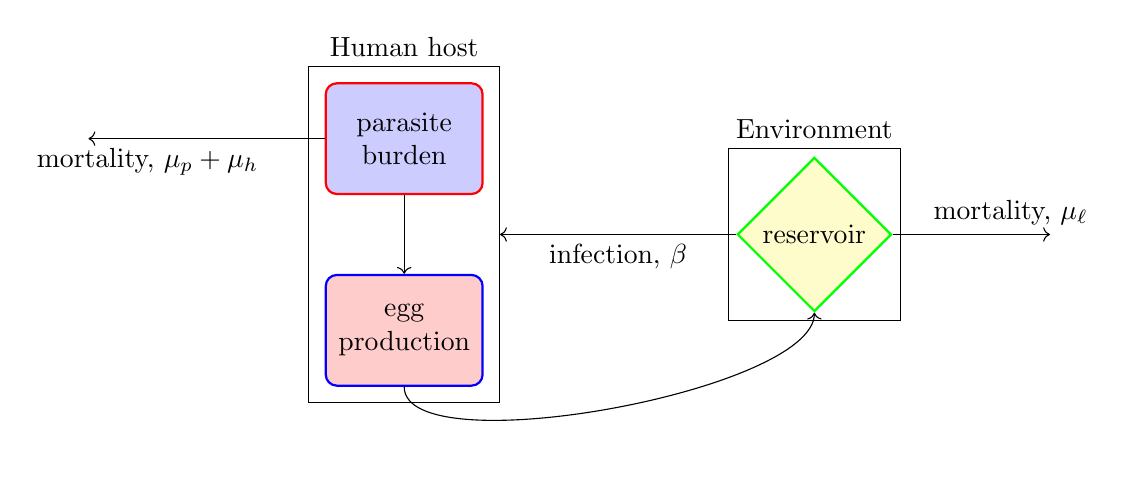
\begin{tikzpicture}[auto]
\tikzstyle{decision} = [diamond, draw=green, thick, fill=yellow!20,
text width=4.5em, text badly centered, inner sep=1pt]
\tikzstyle{block} = [rectangle, draw=red, thick, fill=blue!20,
text width=5em, text centered, rounded corners, minimum height=4em]
\tikzstyle{blockR} = [rectangle, draw=blue, thick, fill=red!20,
text width=5em, text centered, rounded corners, minimum height=4em]
\tikzstyle{line} = [draw, thick, -latex’,shorten >=2pt];
\tikzstyle{cloud} = [draw=red, thick, ellipse,fill=red!20, minimum height=2em];


\node [block] (P) {parasite burden};
\node [blockR,below= of P] (E) {egg production};
\node[draw, fill=pink, fill opacity=0.0,inner xsep=2mm,inner  
ysep=2mm,fit=(P)(E),label={90:Human host}](H){}; % here label command is used to label the block, which covers block D and E.

\node [decision, right=3cm of H] (R) {reservoir};
\node[draw, fill=pink, fill opacity=0.0,inner xsep=1mm,inner  
ysep=1mm,fit=(R),label={90:Environment}](A){}; % he

\node [left=3cm  of P](MP){};
\node [right=2cm of R](MR){};


%Lines
\draw[->] (P.south) -- (E.north) node[right] {};

\draw[->] (E.south) .. controls +(down:10mm) and +(down:10mm) .. (R.south);


%\draw[->] (P.south) -- (E.north) node[right] {};

\draw[->] (P.west) -- (MP.east)  node [near end] {mortality, $\mu_{p}+\mu_{h}$};

\draw[->] (R.east) -- (MR.west)  node [near end] {mortality, $\mu_{\ell}$};

\draw[->] (R.west)  -- (H.east)  node [midway] {infection, $\beta$};







%\matrix [column sep=5mm,row sep=7mm]
%{
%	% row 1
%	\node [cloud] (expert) {expert};
%	\node [cloud,right=3cm  of expert] (expert) {expert};
%	 &
%	\node [block] (init) {initialize model}; &
%	\node [cloud] (system) {system}; \\
%	% row 2
%	& \node [block] (identify) {identify candidate model}; & \\
%	% row 3
%	\node [block] (update) {update model}; &
%	\node [block] (evaluate) {evaluate candidate models}; & \\
%	% row 4
%	& \node [decision] (decide) {is best candidate}; & \\
%	% row 5
%	& \node [block] (stop) {stop}; & \\
%};
\tikzstyle{every path}=[line]
%\path (init) -- (identify);
%\path (identify) -- (evaluate);
%\path (evaluate) -- (decide);
%\path (update) |- (identify);
%\path (decide) -| node [near start] {yes} (update);
%\path (decide) -- node [midway] {no} (stop);
%\path [dashed] (expert) -- (init);
%\path [dashed] (system) -- (init);
%\path [dashed] (system) |- (evaluate);
\end{tikzpicture}	
\end{figure}


\begin{figure}[h]
\centering
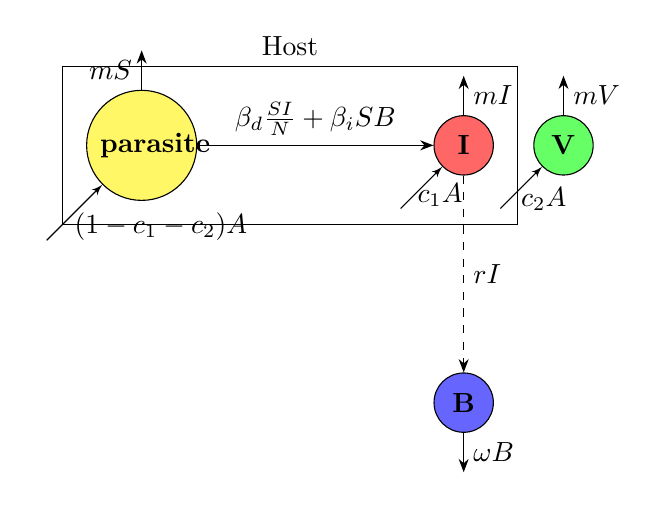
\begin{tikzpicture}
    \node [S] (S) {\textbf{parasite}}; 
    \node [I,right=3cm  of S] (I)  {\textbf{I}};
    \node [V,right=0.5cm of I] (V)  {\textbf{V}};
    \node [bacteria, below=2.5cm of I] (B)  {\textbf{B}};
    \node [below left=1cm of S](ingresosS){}; 
    \node [below left=0.75cm of I](ingresosI){}; 
    \node [below left=0.75cm of V](ingresosV){}; 
    \node [above=0.5cm of S](muertesS){}; 
    \node [above=0.5cm of I](muertesI){};
    \node [above=0.5cm of V](muertesV){};
    \node [below=0.5cm of B](muertesB){};     
 
 
    \draw [arrow] (S) -- node [above] {$\beta_d \frac{SI}{N}+ \beta_i SB$}(I); 
    \path [line] (ingresosS) -- node [below right=-5pt] {$(1-c_1-c_2)A$} (S);
    \path [line] (ingresosI) -- node[ below right=-7pt] {$c_1A$} (I);
    \path [line] (ingresosV) -- node [below right=-5pt] {$c_2A$} (V);
    \draw [arrow, dashed] (I) -- node [right]{$rI$} (B);
    
    \draw [arrow] (S) -- node [left] {$mS$ } (muertesS);
    \draw [arrow] (I) -- node [right] {$mI$} (muertesI);
    \draw [arrow] (V) -- node [right] {$mV$} (muertesV);
    \draw [arrow] (B) -- node [right] {$\omega B$} (muertesB);
    
    \node[draw, fill=pink, fill opacity=0.0,inner xsep=3mm,inner  
    ysep=3mm,fit=(S)(I),label={90:Host}](f){}; % here label command is used to label the block, which covers block D and E.
    
\end{tikzpicture} 
\caption[Figura]{Diagrama de flujo de la dinámica de la transmisión de brucelosis en una población de vacas  de cría adultas.}
\end{figure}




\section{Puntos de equilibrios y número reproductivo básico}

\subsection{Equilibrio libre de infección}
La expresión para el punto de  equilibrio libre de infección se obtiene  resolviendo el sistema formado por las ecuaciones igual a cero (\ref{eq:modS}-\ref{eq:modB})  y teniendo en cuenta que $I=0$ y $B=0$. Luego de algunos cálculos tenemos la expresión general para el equilibrio libre de infección.
  \begin{equation}
P^*_{li} =(S^*_{li},0,V^*_{li},0)= ( (1-c_2)N, \, 0, \, c_2N, \, 0) \label{eq:ELI}
\end{equation}
 Esta familia de puntos de equilibrio existe si $c_1=0$, dado que de otra forma la ecuación (\ref{eq:modI}) no se anularía. Esto nos dice que para que exista un punto de equilibrio libre de infección no debe haber ingreso constante y sostenido de animales infectados. 
 
\subsection{Número reproductivo básico}




\bibliographystyle{acm}
\bibliography{Bibliografia}

\end{document}
